%%%%%%%%%%%%%%%%%%%%%%%%%%%%%%%% 
\section{The Cold Electronics (CE)} 
\label{sec:detectors-fd-ref-ce}

The TPC read-out electronics are referred to as the ``Cold Electronics'' (CE) because they will reside in LAr,
mounted directly on the APA front-end (Figure~\ref{fig:elec_CMBonAPA}).
This will minimize channel capacitance and noise by keeping the length of the connection between an anode wire
and its corresponding electronics input to an absolute minimum.
The CE will be implemented as ASIC chips using CMOS technology,
which performs well at cryogenic temperatures,
and will provide amplification, shaping, digitization, buffering and multiplexing (Mux) of the signals.
\begin{cdrfigure}[The front end electronics as mounted on an APA]{elec_CMBonAPA}{The front end electronics,
shown in the red circle, as mounted on an APA.}
%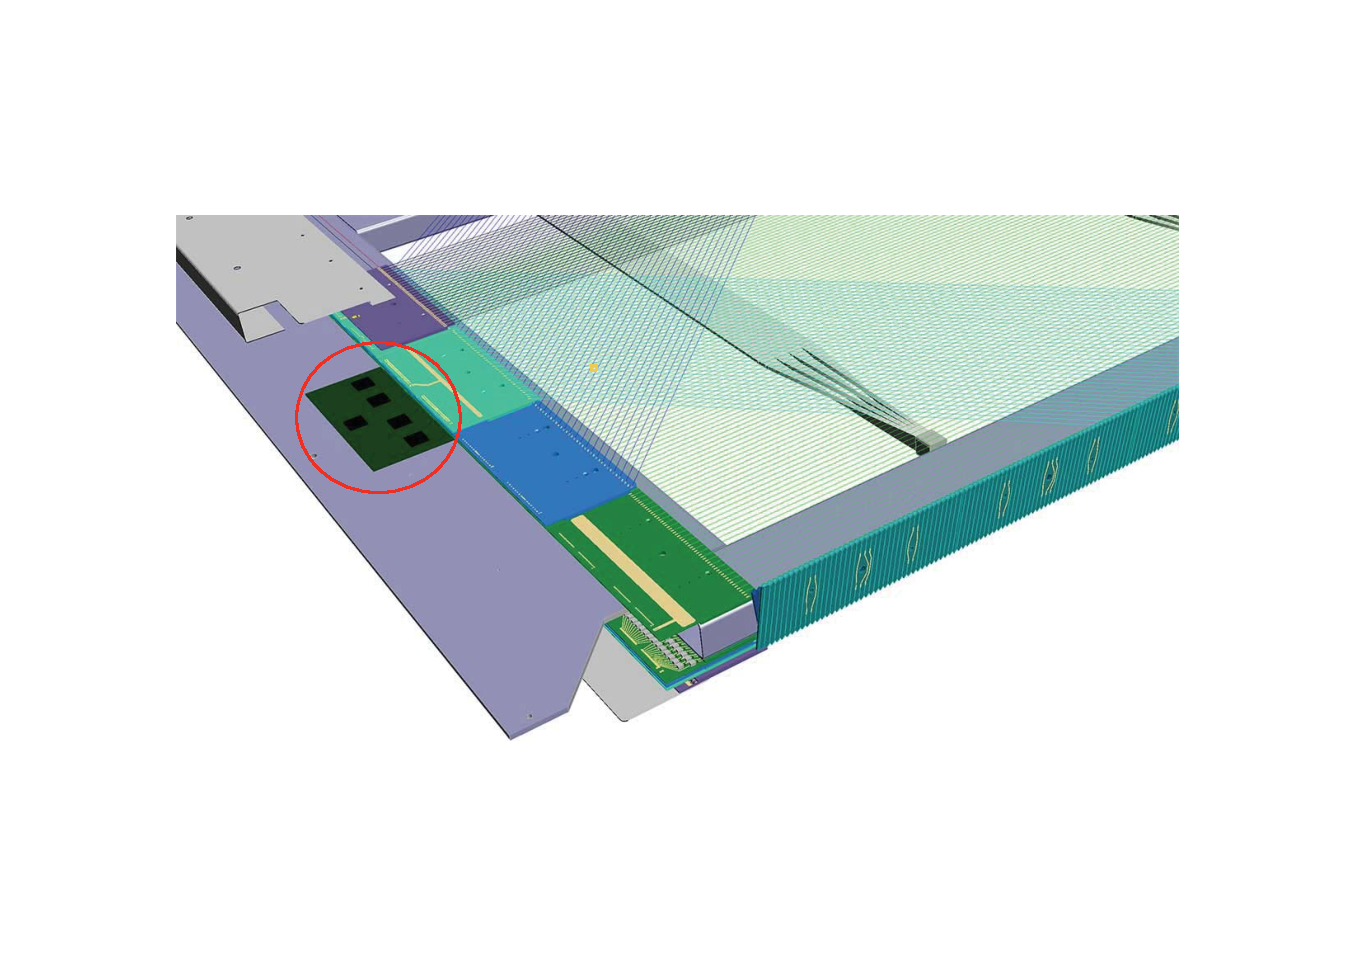
\includegraphics[width=1.00\linewidth]{elec_CMBonAPA_1.pdf}
\end{cdrfigure}

The scope of the CE subsystem includes the design, procurement, fabrication, testing,
delivery and installation of the CE, the principle components of which are:
\begin{itemize}
\item Front-end electronics cards installed on the APAs;
\item Signal feedthroughs mounted on the cryostat;
\item Power supplies and cabling.
\end{itemize}
The most significant requirements for the CE are to:
\begin{itemize}	
\item Read out the TPCs and transmit their data to DAQ;
\item Record the channel waveforms continuously without dead time;
\item Provide sufficient precision and range in the digitization to satisfy the KPP;
\item Operate for the life of the facility without significant loss of function;
\item Use only materials that are compatible with high-purity liquid argon.
\end{itemize}

The CE architecture is manifested in the Cold Mother Board assembly (CMB),
which consists of an analog mother board with a digital ASIC mezzanine (Figure~\ref{fig:elect_schem}).
The analog mother board is instrumented as a 128-channel board which uses eight 16-channel FE ASICs,
eight 16-channel ADC ASICs, low-voltage regulators, and input-signal protection.
The 16-channel FE ASIC provides amplification and pulse shaping.
The 16-channel ADC ASIC comprises a 12-bit digitizer, local buffering,
and an 8:1 Mux stage with two pairs of serial readout lines in parallel.
A Cold Digital Data (COLDATA) ASIC chip mounted on each CMB provides an additional Mux of 4:1 and
is capable of driving the data at 1~Gb/s through 30~m of copper cable to the feedthrough and on to DAQ. 
Each APA is instrumented with 20 CMBs, for a total of 2,560 channels per APA.
\begin{cdrfigure}[The CE Architecture]{elect_schem}{The CE Architecture. The basic unit is the 128-channel CMB}
%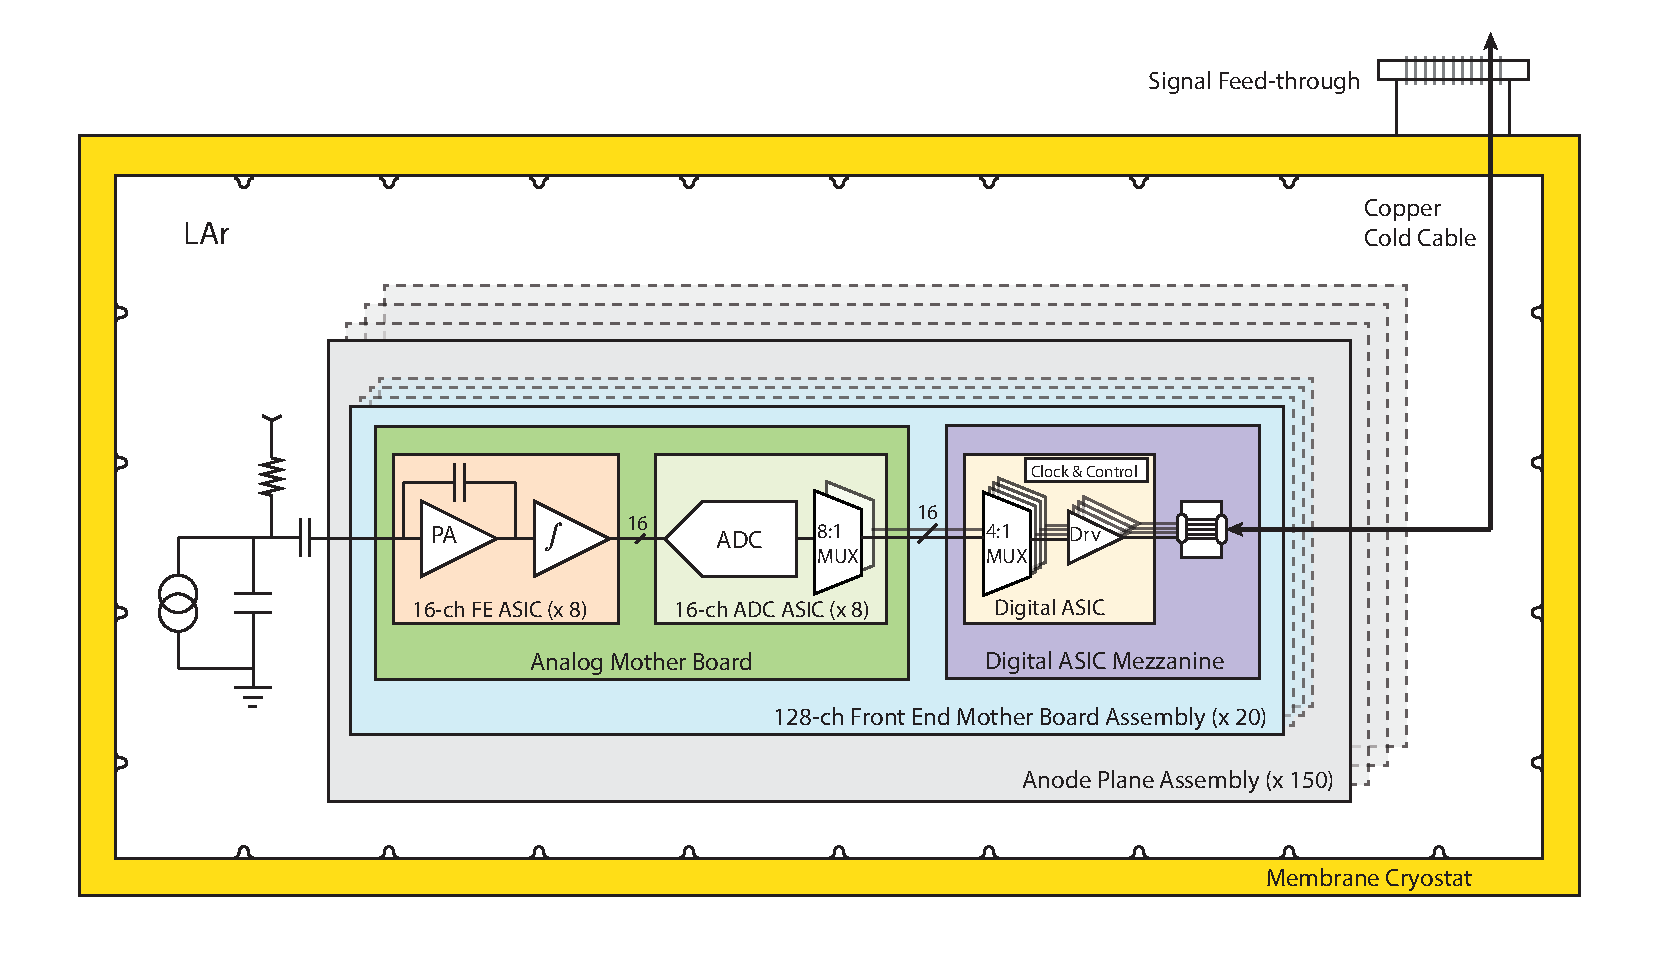
\includegraphics[width=\linewidth]{elect_schem.pdf}
\end{cdrfigure}
\begin{cdrfigure}[Functional Block Diagram of the Cold Digital Data (COLDATA) ASIC]{elec_COLDATAfig}{Functional Block Diagram of the Cold Digital Data (COLDATA) ASIC}
%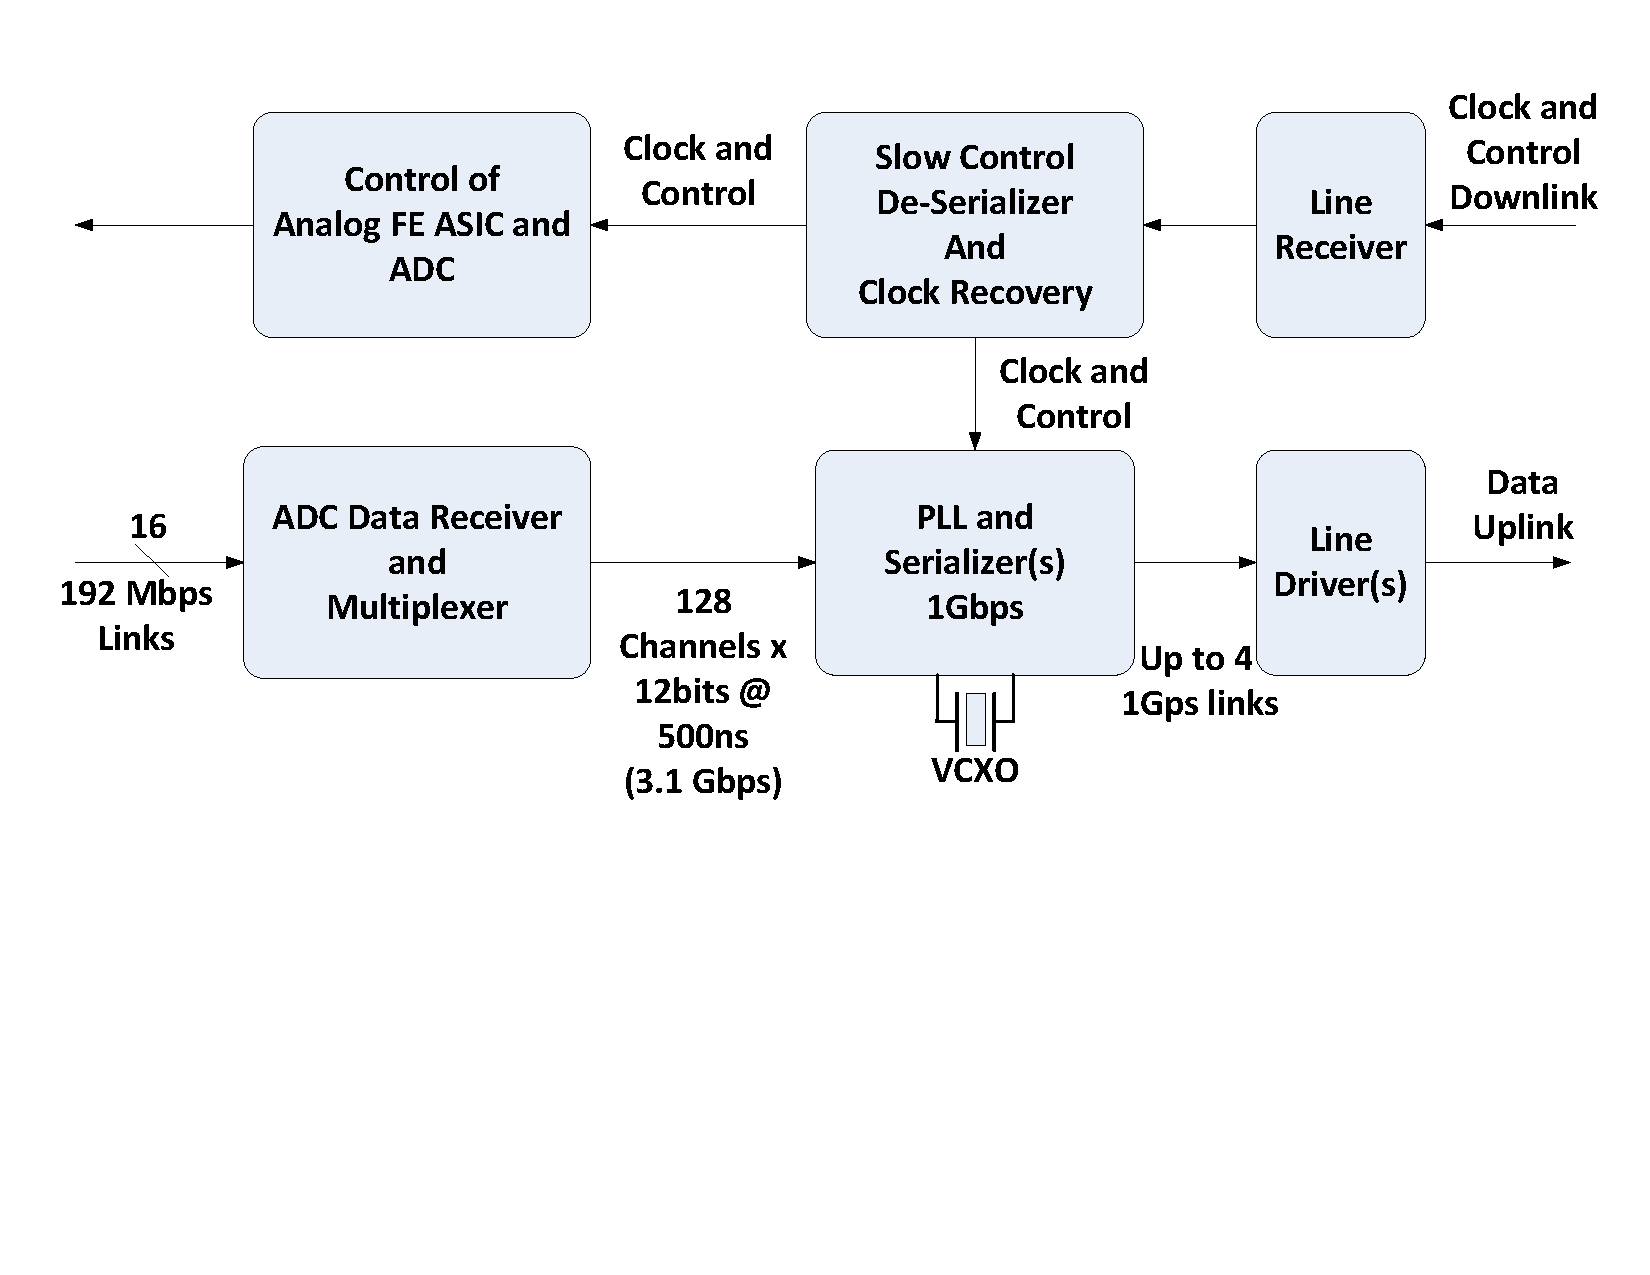
\includegraphics[width=6in]{elec_COLDATAfig.pdf}
\end{cdrfigure}
\fixme{add figures and uncomment}

An important aspect of CMOS technology is that the lifetime at cryogenic temperatures is well-understood and can be
well-controlled, {\em provided that close control is maintained over the implementation details.}
This requirement of close control cannot be satisfied by any commercial device,
where there an ever-present risk of process change in its manufacture.
Strict requirements in industry to deliver a device with equivalent performance and lifetime,
despite a change in the proprietary manufacturing process or technology,
only applies to a range of temperatures which does {\em not} include LAr temperatures.
Accelerated lifetime-testing of commercial devices will not protect against 
a substantially different performance or shorter lifetime in the cold following a manufacturing process change
over which we have no control, nor necessarily any knowledge.
It is because of this serious concern that we are undertaking the development and fabrication of our own devices, 
so that tight control of the process can be maintained.
It is worth noting that the CMB, together with the FE and ADC ASIC chips, has already been prototyped and tested,
using a commercial FPGA to perform the role of the digital ASIC,
which is currently under development.

The 1~Gb/s data rate is not high enough to require the use of optical fibers in the cold,
nor is there a need for zero suppression or data compression.
This greatly reduces the complexity of the COLDATA ASIC, with a corresponding decrease in overall risk,
including risk of failure-to-implement (within a fixed schedule and budget)
and risk of device failure during long-term operation.

% \begin{cdrtable}[short]{cc}{label}{long}  %The third argument (reads {cc}) can use c, l, r or p{some length} 
% Header Column1 & Header Column 2 \\ \toprowrule
% Row 1 & First \\ \colhline
% Row 2 & Second \\ \colhline
% Row 3 & Third \\
% \end{cdrtable}
